\section{Weak Lensing Systematics}

The LSST provides an opportunity to mitigate WL systematics using the observing strategy. This opportunity was not possible in previous surveys because the LSST will be the first survey to dither at large scales (relative to the field of view) with a large number of exposures.

Weak lensing systematics that have coherent shape distortions such as PSF modeling errors and brighter-fatter shape distortions have been observed to have specific directions in single exposures. With a suitable dithering algorithm (both translational and rotational), one can average down these systematics. While the process of averaging them down is more complicated, it strongly correlates with the number of unique observations for a set of simulated, uniformly distributed objects on the sky, restricted to i-band only (which the main weak lensing analysis will use). We, therefore, use the average number of unique i-band visits per object as our metric, with objects generated randomly from a uniform distribution on the sky, after applying a depth (coadded-depth$<26$ at Y10) and extinction ($E(B-V)<0.2$) cut. We specify "unique" observations to ensure that a dithering algorithm is implemented and to penalize strategies that take repeat observations with the same centers of focal plane, which does not help averaging down systematics.

It is essential for these visits to be of high quality. There are already several metrics in MAF that ensure this, the ones that specifically apply are coadded depth (ExgalM5 or CoaddM5), the airmass distribution, and the seeing distribution. More uniform strategies will have narrow distributions. These metrics ensure survey uniformity, which is one of the crucial things that average down WL systematics, and all these metrics are, in one way or another, a measure of uniformity.

Figure~\ref{fig:WLSystematicsRankings} shows the result of this metric for the 16 recent OpSim runs. 

Certain trends can be seen from  figure~\ref{fig:WLSystematicsRankings}: more visits in the main WFD survey are very beneficial for averaging down weak lensing systematics (whether achieved by smaller area, shorter 20-second visits, or single 30-second exposures that reduces total readout time. OpSim runs with more exposure to the galactic planes underperform since the WL analysis will omit the galactic plane due to high extinction, and so less time will be spent on the areas that the WL analysis will use (and less visits per objects since the objects are not placed in the galactic plane). All OpSim rolling cadence runs have bugs that could explain their underperformance in this metric, but we cannot make a general comment on rolling cadence runs until we have analyzed runs without any bugs. Finally, wider area OpSim runs also do worse because using the same amount of time to cover a larger area will decrease the number of visits.

\begin{figure}[htb]
    \centering
    \caption{The metric values as a function of obersving strategy.}
    \label{fig:WLSystematicsRankings}
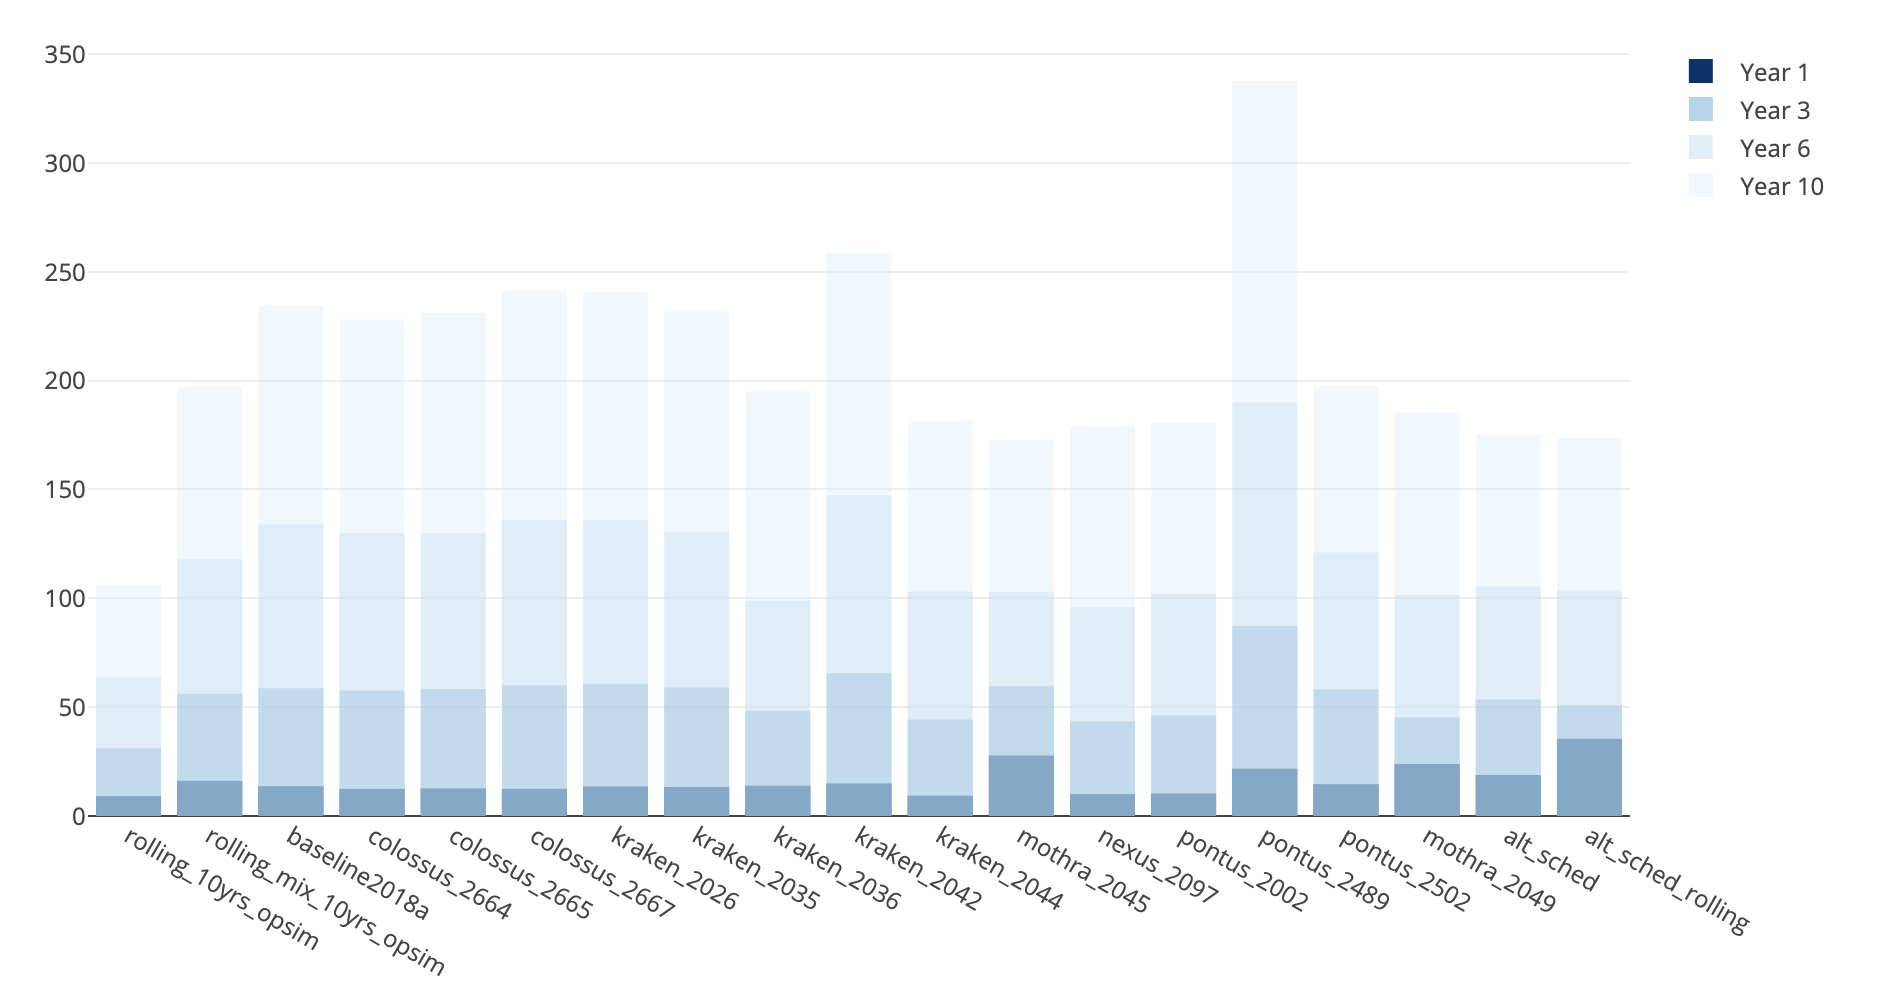
\includegraphics[\textwidth]{../figures/wlsystematicsmetric.png}
\end{figure}

It is important to note that this metric assumes that the dithering algorithm's efficiency is the same for the strategies, where efficiency is defined as the number of uniformly distributed unique positions of visits. This assumption is satisfied when using MAF stackers, but may differ otherwise.
